\chapter{Method}
\label{chap:method}

%\lipsum[100]

The simulation in this paper was performed using the freely available \texttt{REBOUND} multi-purpose collisional N-body framework, developed by \citep{2012A&A...537A.128R}.
%PUT LOTS MORE HERE
%the \texttt{Janus} integrator \citep{2017arXiv170407715R} within the 
\section{Evolution of Earth-impacting cometary bodies in the inner Solar System}
\label{method:evol}
%\subsection{Model Framework}
After $N$ perihelion passages the number $n_N$ of comets that remain bound the Solar System is given by \citep{1976NASSP.393..445E},

\begin{equation}
    n_N \sim \dfrac{1}{2}n_{new}N^{-1/2}~,
    \label{eq:remain_bound}
\end{equation}

where $n_{new}$ is the number of dynamically new comets.

Eq.~\eqref{eq:remain_bound} shows that when considering an initial population of comets injected into the planetary region near Earth at $q \sim 1$ AU, one can expect that upon the first perihelion passage, roughly half the initial population are scattered into interstellar space, and the remainder are set to return as evolved LPCs.

This $N^{-1/2}$ law of survival of comets against hyperbolic ejection is helpful for our understanding of scattered comets evolving through the Solar System. Evolved LPCs spend much longer timescales in the planetary system with a higher probability of migrating towards Earth-crossing orbits, than dynamically new comets falling directly to the Earth from an initial reservoir. A study by \cite{2012MNRAS.423.1674F} estimated from observational data that about 70\% of comets in the LPC population with $q < 1.3$ AU are dynamically evolved, indicating that evolved comets outnumber dynamically new comets in the near-Earth region. 

Because of this, we performed a numerical integration to model the dynamical cometary evolution in the inner Solar System. This allows one to consider the evolved impact flux reaching Earth. The physics of cometary physics decay mechanisms and other non-gravitational processes eg. outgassing, effects of solar wind were deemed negligible for the purpose of this research, as gravitational forces were taken to most dominant in determining the paths of comets through the Solar System.

Our numerical simulation involved a reverse-step integration examining the orbital migration of Earth-impacting cometary bodies in the Solar System.
The purpose of this was to generate simulation information on the orbital history of the cometary bodies, back from their Earth-impacting trajectories to points in their early dynamical lifetimes. This would help inform us on the nature of the cometary bodies' dynamical lifetimes and the various transfer mechanisms responsible for transporting them into the inner Solar System towards Earth. The framework for our simulation model is as follows:

The simulation was performed using \texttt{MERCURIUS} - a hybrid integrator available in \texttt{REBOUND} that smoothly transition between the \texttt{WHFAST} \citep{2015MNRAS.452..376R} and \texttt{IAS15} \citep{2015MNRAS.446.1424R} algorithms - making it ideal for modelling highly eccentric orbits in a planetary environment. Both \texttt{WHFAST} and \texttt{IAS15} preserve properties specific to a Hamiltonian system; that is they preserve the symplecticity. Because we neglect planetary collisions, the Solar System can described as Hamiltonian in this simulation and therefore benefit from the use of these two integrators in relation to long-term energy conservation.

We included the Sun and all 8 planets of the Solar System - with the exclusion of their natural satellites. This was a decision taken to minimise computation time, as the short orbital periods of the natural satellites would have placed constraints on the integration time-step of our simulation. The gravitational effects of the natural satellites were assumed to have a negligible effect on the test particles throughout the course of the integration. Furthermore, there was a low prospect for collisions or encounters between test particles migrating through the Solar System and these natural satellites, due to their relatively low mass and sizes in comparison to the planets.

However, the assumption described does not hold true for the Moon - which plays an important role in Earth's dynamics. Due to the nature of this simulation involving Earth-impacting bodies, the effect of the Moon needed to be modelled appropriately. We therefore employed Newton's shell model to approximate the Earth-Moon system as a sphere of total radius $4\times10^5$ km, of combined mass $m_{earth}+m_{moon}$, with the centre of this sphere positioned at the centre of mass of the Earth-Moon system, orbiting in place of the Earth. This shell model consideration was able to improve computation times, by eliminating the need for short integration time steps that reflect the Moon's short orbital period in comparison to the planets. Additionally, a gravitational softening length equal to Earth-Moon system's radius was chosen.

\subsection{Initial Conditions}

We parametrised the initial conditions of the Solar System at the present epoch by describing the positions in space of all objects in our simulation with cartesian coordinates $(x,y,z)$, and velocity components $(v_x, v_y, v_z)$. Our values for position and velocity were taken to be the state of the Solar System at 01-12-2017 12:00 UTC - given by data sourced from the NASA JPL Horizons database\footnote{https://ssd.jpl.nasa.gov/horizons.cgi}.

We initialised the positions of Earth-impacting bodies by generating an isotropically distributed population of test particles on the surface of the Earth-Moon system. The test particles were chosen to be massless and collision-less -  this was due to the negligible masses of asteroids and comets in comparison to the larger planets, and the low probability of a collision between a small body and a planet. The choice for these test particles has the additional benefit of leading to a reduction in computation times.

Due to the extraordinarily sensitive starting conditions for N-body simulations of this nature, a Monte Carlo approach was adopted to generate $10^4$ test particles in an isotropic distribution. By randomly selecting initial orbital configurations for each test particle, the same overall final simulation result of the whole ensemble within a certain statistical tolerance could be rediscovered in repeat simulations.

\cite{shoemaker1962interpretation} has shown that for a gravitating body, the most probable impact angle is 45$^\circ$. Additionally, most studies involving planetary cratering rates assume that there is no spatial variation in meteor impact flux, and that the impact velocity and impact angle distributions are independent of position. Because of this, and due to the nature of the isotropic source of LPCs, we initialise our simulation so that there is an isotropic distribution of comets in a sphere around the Earth-Moon system.

We generate the initial $(x,y,z)$, coordinates for each test particle, by selecting values for the polar angle $\theta$ and azimuthal angle $\phi$ subject to the constraints,

\begin{equation}
  \begin{gathered}
    \theta = \cos^{-1}(2u-1); \, 0 \leq u \leq 1~, \\
    0 \leq \phi \leq 2\pi~,
\end{gathered}  
\end{equation}

where $u$ and $\phi$ are randomly and uniformly selected from within the stated ranges. We then transform to cartesian coordinates using,

\begin{equation}
\begin{split}
    x &= R\sin{\theta}\cos{\phi}~, \\
    y &= R\sin{\theta}\sin{\phi}~, \\
    z &= R\cos{\theta}~.
\end{split}
\end{equation}

where $R$ is taken to be $4\times10^5$ km (the radius of the Earth-Moon system). 

\subsection{Velocity Distribution}

%USE https://arxiv.org/pdf/1802.05034.pdf WHEN DESCRIBING VELOCITY DISTRIBUTION PEAKS

Numerous meteoroid velocity distributions have been derived from observations of meteors in Earth's atmosphere (eg. \citep{HUNT200434} with the use of high-gain radar). However these distributions are made up of poor cometary statistics and are liable to underestimations in the number of high velocity, fragmentation-prone meteoroids.

Because of this, we generated a synthetic velocity distribution for Earth-impacting LPCs. This was modelled using a Monte Carlo simulation, assuming an isotropic parabolic source distribution. Using the method described by \cite{2000MNRAS.315..629H}, assuming that the Earth is moving at a constant velocity in a circular orbit, the expected comet-Earth collision velocities $V_i$ were extracted from this synthetic population of comets using,

\begin{equation}
    V_i^2 = \sqrt{\dfrac{2GM_\Earth}{R_\Earth}} + GM_\odot \left(\dfrac{3}{r_\Earth}-2 \sqrt{\dfrac{p}{r_c^3}} \cos i - \dfrac{1}{a}\right) ~,
    \label{eq:im_vel}
\end{equation}

where $M_\Earth$ and $M_\odot$ are the masses of the Earth and Sun respectively, and $r_\Earth$ and $r_c$ are the radii of the Earth's and comet's orbits respectively ($r_\Earth = 1$ AU). $p$, $a$ and $i$ are the semi-latus rectum, semi-major axis, and inclination elements of the comet's orbit respectively, and $R_\Earth$ is the radius of the Earth. The gravitational influence of the Moon on incoming meteoroids was taken to be negligible in comparison to the Earth - so no additional considerations were taken for the generated Earth-impact velocities prior to launching test particles from the surface of the Earth-Moon system.

\begin{figure}[t!]
    \centering
    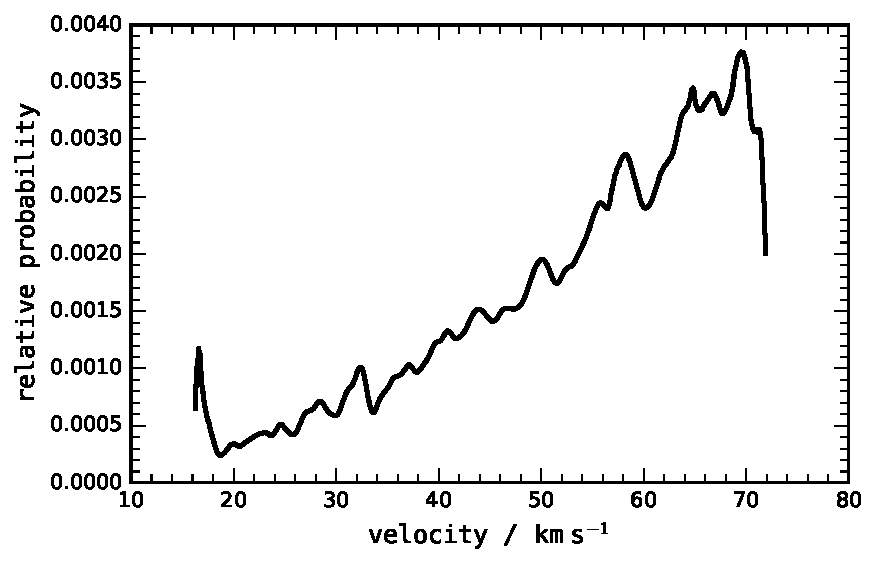
\includegraphics{vel_dist.pdf}
    \caption[Velocity distribution of Earth-impacting cometary meteoroids]{Synthetic impact velocity distribution of LPC meteoroids at the Earth.}
    \label{fig:vel_dis}
\end{figure}

\iffalse
\begin{figure*}[t!]
    \centering
    \begin{subfigure}[t]{0.5\textwidth}
        \centering
        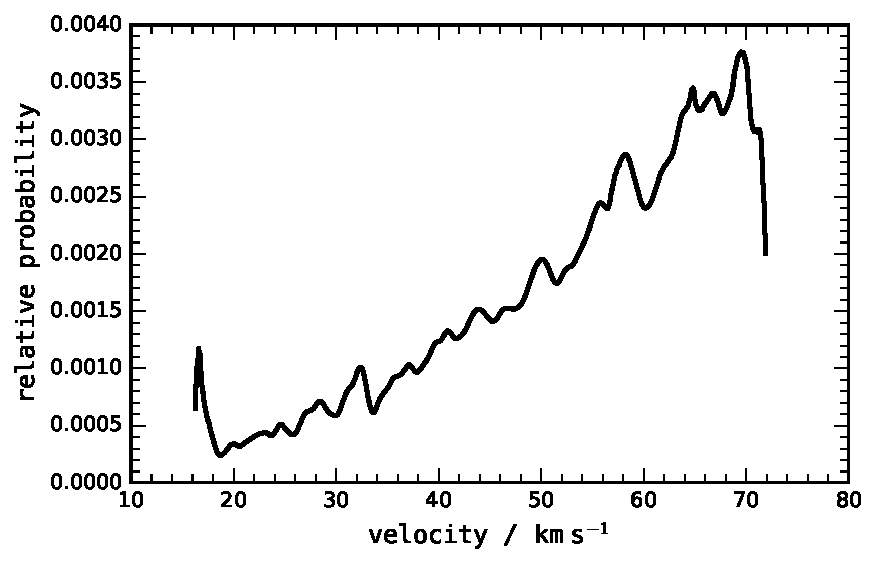
\includegraphics[width=1\linewidth]{vel_dist.pdf}
        \caption{Lorem ipsum}
    \end{subfigure}%
    ~ 
    \begin{subfigure}[t]{0.5\textwidth}
        \centering
        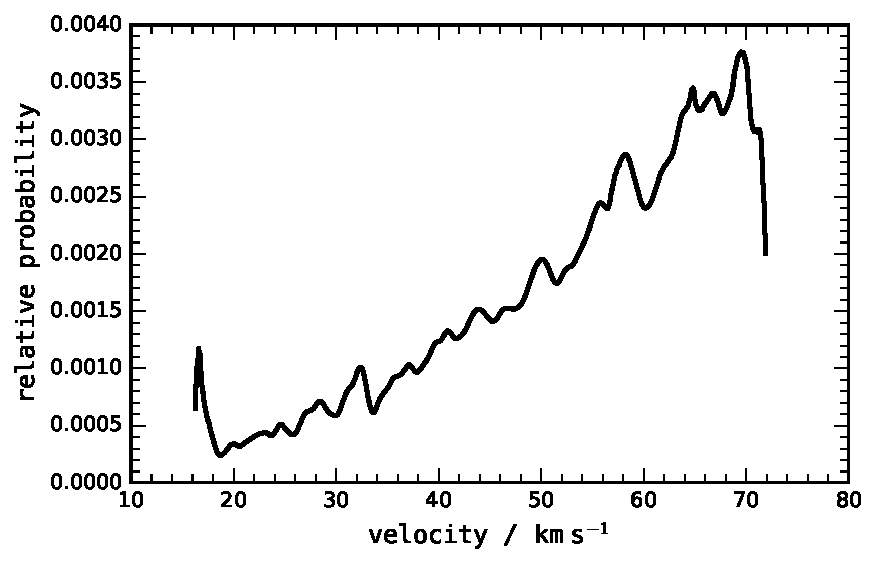
\includegraphics[width=1\linewidth]{vel_dist.pdf}
        \caption{Lorem ipsum, lorem ipsum,Lorem ipsum, lorem ipsum,Lorem ipsum}
    \end{subfigure}
\end{figure*}
\fi

Fig.~\ref{fig:vel_dis} shows the synthetic Earth impact velocity distribution for LPCs. We see that the plot exhibits a peak at both ends of the distribution. These represent the two different extremes of a comet-Earth impact - where a comet is orbiting on the same plane as the Earth and collides on either a prograde or retrograde approach. 

By considering an Earth-impacting comet, with an aphelion very far from the Sun, one can use the escape velocity $v_{esc}$ of the Sun for the comet orbiting on the plane of the ecliptic at 1 AU. Using $v_{esc}=\sqrt{2GM_{\odot}/r}$ where $M_{\odot}$ is the mass of the Sun and $r$ is the distance from the Sun to the comet, the maximum speed for a cometary body impacting the Earth is 42.2 km$\,$s$^{-1}$. This is the maximum velocity for an Earth-approaching comet - otherwise it would not be gravitationally bound to the Solar System. 

By considering a head-on Earth impact as well as an Earth-impact facing the planet behind its direction of travel, the minimum and maximum cometary impact velocities are given by,

\begin{equation}
    (\sqrt{2}-1) \sqrt{ \dfrac{GM_{\odot}}{1 \,\mathrm{AU}} } \leq |v_i| \leq (\sqrt{2}+1) \sqrt{\dfrac{GM_{\odot}}{1 \,\mathrm{AU}}} ~.
\end{equation}
 
These bounds for a cometary meteoroid distribution support the synthetic result shown in Figure.~\ref{fig:vel_dis}. Furthermore, the mean impact velocity is 54 km$\,$s$^{-1}$, in agreement with 53 km$\,$s$^{-1}$ reported by \cite{1988merc.book..274S} for LPC impacts. The calculated distribution was therefore accepted as an appropriate characterisation of impacting comets' velocities for use in the simulation.

%By considering the escape velocity $v_{esc}$ of the Sun for an object orbiting on the plane of the ecliptic at 1 AU, one can use $v_{esc}=\sqrt{2GM_{\odot}/r}$ where $M_{\odot}$ is the mass of the Sun and $r$ is the distance from the Sun to the comet, to calculate the minimum and maximum speeds for a cometary body impacting the Earth. By considering a head-on Earth impact as well as an Earth-impact facing the planet behind its direction of travel - an initial choice for the launch velocity $v$ of each test particle was then selected - such that in the reference frame of the Solar System, the condition $12.4$ km$\,$s$^{-1} \leq |v| \leq 71.9$ km$\,$s$^{-1}$ held true. The absolute minimum and maximum velocity of a cometary meteoroid represent cases where the comet resided on the plane of the ecliptic. This is an unlikely scenario as, for example, LPCs are isotropically distributed. Therefore further selections on velocities were required in order to adequately model the lower expectations for higher-velocity impacts in this range.

%We achieved this by fitting a curve to a meteoroid velocity distribution by \cite{HUNT200434}. This distribution was based on data from the Canadian Meteor Orbit Radar (CMOR) \citep{2014pim3.conf...84W}, which had a large sample size ($>$ 3000) of high velocity meteoroids, making the statistics more reliable for cometary meteoroids.

%The distribution was replicated by fitting two Gaussian distribution functions to the data from \cite{HUNT200434} (See Figure.~\ref{fig:vel_dis}). In order to replicate the distribution, the first Gaussian fit was used for the range 17 km$\,$s$^{-1}$ to 48 km$\,$s$^{-1}$ and the second Gaussian fit was used in the range 48 km$\,$s$^{-1}$ to 72 km$\,$s$^{-1}$.

%The requirement for two curves needing to be fit to the distribution was assumed to be indicative of asteroid and cometary meteoroids. Due to the difficulties in extracting the cometary velocity distribution alone - the velocity distribution representative of all asteroidal and cometary meteoroids was chosen. A filtering mechanism was then employed at the conclusion of the simulation based on dynamical characteristics, in order to extract the cometary population alone (detailed in \S~\ref{chap:results}). For each particle, the velocity of the Earth-Moon system was summed onto a velocity sampled from this replicated distribution.

For each test particle in the simulation, an initial choice of velocity was randomly selected from the generated distribution. Additional final considerations were then applied to the selected velocities. Due to the nature of the random sampling of velocities and positions it was, for example, entirely possibly for a test particle to be assigned a position on the surface of the Earth-Moon system with a velocity vector that caused it to fall towards the Earth upon a reverse-step integration. As this is not the intended behaviour for this simulation of Earth-impacting comets, additional checks were required. If the velocity vector was directed inside the Earth-Moon system, the test particle's location and velocity was reselected. Additionally, if the magnitude of the velocity vector (when summed to the velocity of the Earth-Moon system) exceeded 72 km$\,$s$^{-1}$, the velocity vector was rejected and a new one selected.

\clearpage
\subsection{Launching Routine}

In order to replicate impactors arriving at Earth at different time periods, the population of test particles were gradually released over a time period of 12 yrs. The time period for launches was determined by a random generator using a normal distribution.  The reason for this decision was because Jupiter plays one of the most important roles in influencing the orbits of small bodies in the Solar System - and releasing the test particles over a time period similar to the orbital period of Jupiter was an important decision to help replicate the various different gravitational interactions small bodies have with Jupiter at different points in its orbit.

The Solar System is chaotic, with a Lyapunov timescale of $\sim 5$ Myr \citep{1996CeMDA..64..115L}. A time period of 10 Myr was chosen to be the length of the simulation, in order to fully capture a period of Solar System stability. The integration routine ran with a reverse time step of 6 days, with data snapshots taken every 500 years. At each snapshot the orbital parameters of each simulated body were recorded and written to a .hdf5 file for later analysis. The length of our integration was chosen such that there was not an unnecessarily large expenditure of computing resources, while physically meaningful results were still produced.

\begin{figure}[t!]
    \centering
    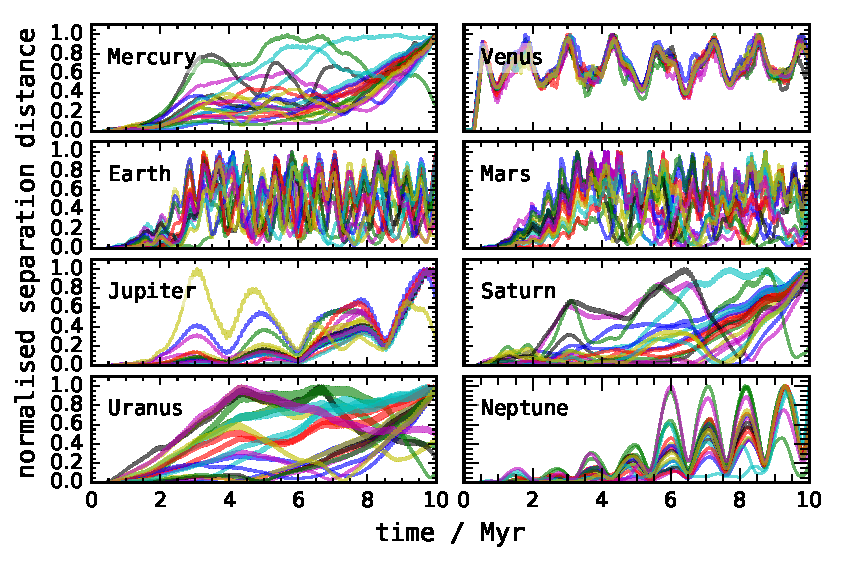
\includegraphics{info_loss.pdf}
    \caption[Parallel Simulations]{(Heavily smoothed) normalised separation distances for each planet in each simulation, from the positions of the planet in the first simulation.}
    \label{fig:info_loss}
\end{figure}

\clearpage
\subsection{Numerical Accuracy}
\label{sec:accuracy}

The nature of the simulated test particles meant that they only gravitationally interacted with the planets, and not with each other. Additionally, the computation time for an N-body simulation scales with the amount of particles. Therefore, in the interests of computational and storage constraints, the simulation was executed as a set of 21 parallel simulations, considering the ejection of $\sim2\times10^{4}$ particles in total.

Chaotic systems such as the Solar System are extraordinarily sensitive to initial conditions. Therefore, position differences on the order of metres between two simulations can lead to completely different dynamical system configurations after $\sim5$ Myr. A lack of robustness between results does not necessarily mean an N-body integration does not accurately represent reality. However, it does mean that for the scope of this investigation we explore the various dynamical pathways explored by comets integrated backwards in time, and are not concerned with retracing the comets' paths continuously back to their source reservoirs.

Because of rounding errors incurred due to floating point operations in the \texttt{MERCURIUS} integrator, the evolution of planets across all the simulations did not perform identically. Fig.~\ref{fig:info_loss} examines the discrepancies in the positions of the planets across all the simulations. The maximum absolute separations for each planet ranged from a minimum of $4.5\times10^{-5}$ AU (Mercury) to a maximum of 0.14 AU (Jupiter). This suggests that the information losses involved are due to a difference in orbital phase, and not due to substantial differences in position.

A large divergence is observed at the 2.5 Myr for most planets, with the notable exception of Venus. One possible explanation for this behaviour is that this sudden growth is due to a resonant interaction with the giant planets.

The divergences across the simulations does not compromise the output data when analysed as a whole. Each simulation represents a unique Solar System environment, where the the changes in comet orbits are consistently governed by the same dynamics throughout. 

Across all the simulations used in this investigation, the mean relative energy error was maintained at $10^{-7}$. Due to the choice of timestep, the energy error throughout the integrations were characterised by an unbiased random walk caused by round-off errors in floating-point calculations. There were some instances of significant energy jumps (still of order $10^{-7}$). This was assumed to be due to very close encounters with major planets that were not properly resolved.

\iffalse
\begin{figure}[t!]
    \centering
    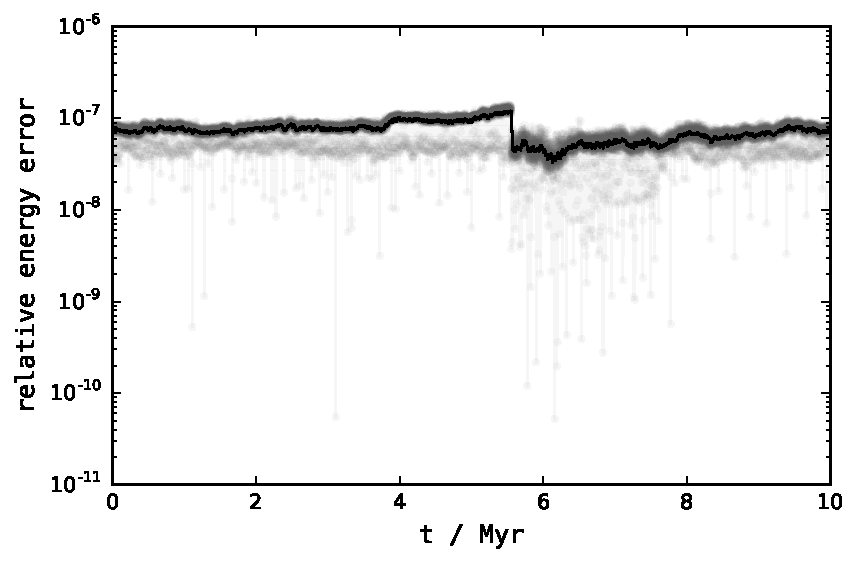
\includegraphics{error.pdf}
    \caption[]{}
    \label{fig:error}
\end{figure}
\fi

\iffalse
\section{Simulating Earth observations of an impending comet impact}

\begin{equation}
    m = H + 5\log(r_{hel}r_{geo}) - 2.5\log(\phi(\theta))~.
\end{equation}
\fi



\iffalse

\subsection{Generating a synthetic population of hazardous long-period comets}

We first generate a synthetic population of hazardous long-period comets, by creating a population of comets subject the following orbital constraints on semi-major axis $a$, inclination $i$ and perihelion distance $r_p$,

\begin{equation}
    \begin{gathered}
        2000 \text{ AU} \leq a \leq 100,000 \text{ AU}~,\\
        0^{\circ} \leq i \leq 180^{\circ}~\\\
        6 R_\odot \leq r_p \leq 1 \text{ AU}~.
    \end{gathered}
\end{equation}

The resulting orbits were then modified further so that they become Earth-impacting. This is carried out by first finding a value of $\theta$ such that $f(\theta)$ is minimised where,

\begin{equation}
    f(\theta) = | \, r_{\Earth} - ||\vec{r}(M = \theta, \omega = 0, a, e, i, \Omega)|| \, | ~,
\end{equation}

and,

\begin{equation}
   r_{\Earth} = ||\vec{r}(M_{\Earth}=\Omega, \omega_{\Earth}, a_{\Earth}, e_{\Earth}, i_{\Earth}, \Omega_{\Earth})||~,
\end{equation}

where $r$ is the distance between the object and the Sun.

A value for $\phi$ is then found such that $f(\phi)$ is minimised where,

\begin{equation}
    g(\phi) = | \, \vec{r}(M = \theta, \omega = \phi, a, e, i, \Omega) \cdot \vec{z} \, | ~,
\end{equation}

where $\vec{z}$ is the Earth's orbital normal vector.

A random lead time $t_l$ is then found, subject to constraints. The comet's and Earth mean anomalies are set to $M = \theta^{\prime}$ and $M_{\Earth} = \theta^{\prime}_{\Earth}$ respectively,

\begin{equation}
    \begin{split}
        \theta^{\prime}_{\Earth} &= \Omega - \dfrac{t_l \sqrt{GM_\odot}}{2\pi {a_{\Earth}}^{3/2}}~, \\
        \theta^{\prime} &= \theta - \dfrac{t_l \sqrt{GM_\odot}}{2\pi {a_{a}}^{3/2}}~.
    \end{split}
\end{equation}

where $M_\odot$ is the mass of the Sun.

\fi